\documentclass[tikz,border={10pt 60pt 10pt 10pt}]{standalone}
\usetikzlibrary{decorations.pathmorphing}
% ---------- begin definition xraytube, headtop and 3-level objects
%
% inspired by the comment of samcarter https://tex.stackexchange.com/users/36296
% to my post https://tex.stackexchange.com/questions/713645
% ---------- definitions for lengths of different segments, scaling,
% and rotation angles.
\def\scl{.4}
\def\wda{1}
\def\wdb{2}
\def\wdc{4}
\def\rotm{40}
\def\rotd{-40}
% ---------- definition for drawing an xray tube
\def\xraytube
{%
  \begin{scope}[scale=\scl, opacity=1, line width=.05cm,
    rounded corners=5pt, transform shape, overlay]
    \draw[gray, bottom color=gray, top color=gray!25] (-\wda,0)  --++(-90:\wdc)
       --++(180:\wdb) --++(-90:\wdb) --++(0:\wdb)   --++(0:\wda) --++(0:\wda)
       --++(0:\wdb)   --++(90:\wdb)  --++(180:\wdb) --++(90:\wdc)  --cycle;
    \draw[gray, top color=gray, bottom color=gray!40] (0,-.35) 
      ellipse (1. and 0.5);
\end{scope}
}%
% ---------- definition for drawing a head viewed from the top
\def\headtop
% ---------- modified form https://tex.stackexchange.com/a/74176/213 
% by Tom Bombadil https://tex.stackexchange.com/users/7279
{%
\begin{scope}[scale=2*\scl, line width=.05cm, rounded corners=3pt,
    rotate=0, looseness=1.,overlay]
  \coordinate   (o) at (0,0) {};
  \coordinate  (or) at ([shift={(0.:4.)}]o.center);
  \coordinate  (ot) at ([shift={(86.:1.)}]o.center);
  \coordinate (ort) at ([shift={(95.:1.)}]or.center);
  \coordinate   (x) at ([shift={(56.5:3.6)}]o.center);
  \coordinate  (xt) at ([shift={(90:.3)}]x.center);
  \coordinate  (xl) at ([shift={(180:.34)}]x.center);
  \coordinate  (xr) at ([shift={(0:.34)}]x.center);
%
  \draw[brown, bottom color=brown!60!orange!25!white, top color=brown!60]
    (xl.center) to [out=40,  in=-140] (xt.center)
                to [out=-40, in=140]  (xr.center);
%
  \draw[brown, right color=brown!60!orange!25!white, left color=brown!60]
    (o.center) to [out=-170, in=160] (ot.center);
%
  \draw[brown, left color=brown!60!orange!25!white, right color=brown!60]
    (or.center) to [out=-10, in=20] (ort.center);
%
  \draw[brown, inner color=brown!60!orange!25!white, outer color=brown!60]
    (o.center) arc (180:360:2) to[out=90, in=0] (x.center)
    to [out=180, in=90] (o.center) -- cycle;
\end{scope}
}%
% ---------- subjects in 3 levels in the head%inspired by the comment of 
% Black Mild https://tex.stackexchange.com/users/140722
% to my post https://tex.stackexchange.com/questions/713739
%---------- definitions for drawing circles, rectangles, and triangles
\tikzset{
  crcl/.pic = {
    \draw[line width=.06cm, red, fill=red] (0,.25) circle (.25cm); },
  rctng/.pic = {
    \draw[line width=.06cm, blue, fill=blue] (0,0) rectangle ++(0.5,0.5); },
  trngl/.pic = {
    \draw[line width=.06cm, green!70!black, fill=green!70!black] (0,0)
      -- ++(60:.6) -- +(-60:.6) -- cycle; },
  % ---------- definition for drawing an xray beam
  rayr/.pic = {
    \draw [decorate, -latex, line width=.05cm] (0,0) -- ++(90:5.2cm); },
  % ---------- definition for drawing an xray field
  raytrg/.pic = {
    \draw[gray, outer color=gray!75, inner color=gray!30] (0,0)
      -- +(110:6.8) -- +(70:6.8)--cycle; },
  %---------- definition for drawing an xray film
  flm/.pic = {
    \draw[gray, top color=gray!80, bottom color=gray!80, middle color=gray!40]
     (0,0) rectangle +(5.,-.2) node[midway]{.}; }
}
% end definition xraytube, headtop and 3-level objects
%
\begin{document}
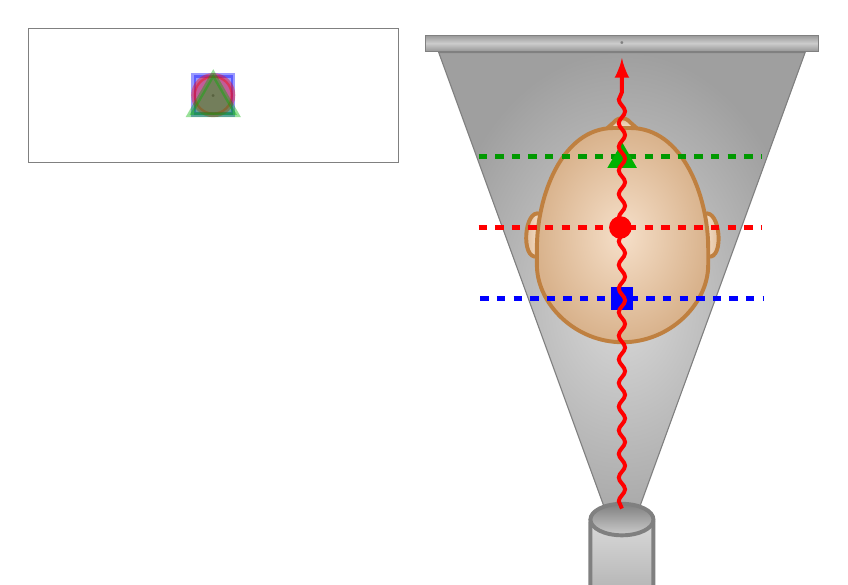
\begin{tikzpicture}
  \pic[shift={(.04cm,.01cm)}] {flm};% The x-ray film
  \pic[shift={(2.54cm,-6.6cm)}] {raytrg};% The x-ray field
  % The head viewed from the top:
  \begin{scope}[shift={(1.46cm,-2.8cm)}, scale=.68]
    \headtop
  \end{scope}
  % The x-ray tube:
  \begin{scope}[shift={(2.54,-6cm)}]
    \xraytube
  \end{scope}
%
% ---------- Drawing subjects in 3 coronal levels in the head
  \begin{scope}[scale=.45, transform shape, shift={(1.6cm,-7.4cm)}]
    \begin{scope}[yshift=2cm]
      \draw[line width=.06cm, red, dashed] (0,0) -- ++(0:8cm);
      \foreach \x in {4} \pic at (\x,-.25) {crcl};
    \end{scope}
    %
    \begin{scope}[xshift=-.2cm]
      \draw[line width=.06cm, blue, dashed] (.25,0) -- ++(0:8cm);
      \foreach \x in {4} \pic at (\x,-.25) {rctng};
    \end{scope}
    %
    \begin{scope}[shift={(-.25cm,4cm)}]
      \draw[line width=.06cm, green!60!black, dashed] (.25,0) -- ++(0:8cm);
      \foreach \x in {4} \pic at (\x,-.25) {trngl};
    \end{scope}
  \end{scope}
  % The x-ray beam direction
  \begin{scope}[decoration={snake, amplitude=.4mm, segment length=3mm,
    post length=4mm}, shift={(2.54cm,-6cm)}]
    \pic at (0,0) [rotate=0, red, scale=1.1] {rayr};
  \end{scope}
  % representation of the shadows of the 3-level subjects on the x-ray film
  \begin{scope}[shift={(-5cm,.1cm)}]
    \draw[gray] (0,0) rectangle +(-20:5) node[midway](mid){.};
  \end{scope}
  \begin{scope}[shift={(-2.9cm,-1cm)}, opacity=.4]
    \pic {rctng};
    \hskip .25cm
    \pic {crcl};
    \hskip -.3cm
    \pic {trngl};
  \end{scope}
\end{tikzpicture}
\end{document}